\documentclass[12pt,a4paper]{article}
\usepackage[utf8]{inputenc}
\usepackage[swedish]{babel}
\usepackage{amsmath}
\usepackage{amsfonts}
\usepackage{amssymb}
\usepackage[affil-it]{authblk}
\usepackage{subcaption}
\usepackage[innercaption]{sidecap}
\usepackage{floatrow}
\usepackage{movie15}

\RequirePackage{color,graphicx}
\usepackage{hyperref}
\definecolor{linkcolor}{rgb}{0,0.2,0.6}
\hypersetup{colorlinks,breaklinks,urlcolor=linkcolor,linkcolor = linkcolor} 
\usepackage{blindtext}
\graphicspath{{C:/Users/danne/Pictures/}}

\begin{document}

\author{Rasmus Svensson%
  \thanks{E-mail: \href{mailto:rasmus.sjobol@gmail.com}{rasmus.sjobol@gmail.com}}, \ {Daniel Holmkvist%
  \thanks{E-mail: \href{mailto:dh222kd@student.lnu.se}{dh222kd@student.lnu.se}}}}
\title{Inlämningsuppgift 1 - 1DV005}
\maketitle
\tableofcontents
\newpage
\section{Scratchuppgifter}
\subsection{Uppgift 1: Euklides algoritm}
PROBLEMLÖSNINGSSTRATEGI 
Vår implementation börjar med att fråga användaren om två tal a,b (här används  Då vill vill att $ a \geq b$ byter vi värde på dem ifall detta ej uppfylls. Sedan använder vi (pseudokod): 
\\
WHILE b != 0         \\
 	rest = a mod b \\
	a = b \\
	b = rest \\ 
	
Vi använder oss av modulus för att beräkna resten, sedan genomför vi helt enkelt Euklides algoritm tills resten från divisionen mellan a och b är 0. Euklides algoritm säger att när resten är 0 är svaret funnet och är a, så där slutar vi med loopen, och skriver ut svaret. \\

%\noindent\begin{minipage}{0.3\textwidth}% adapt widths of minipages to your needs
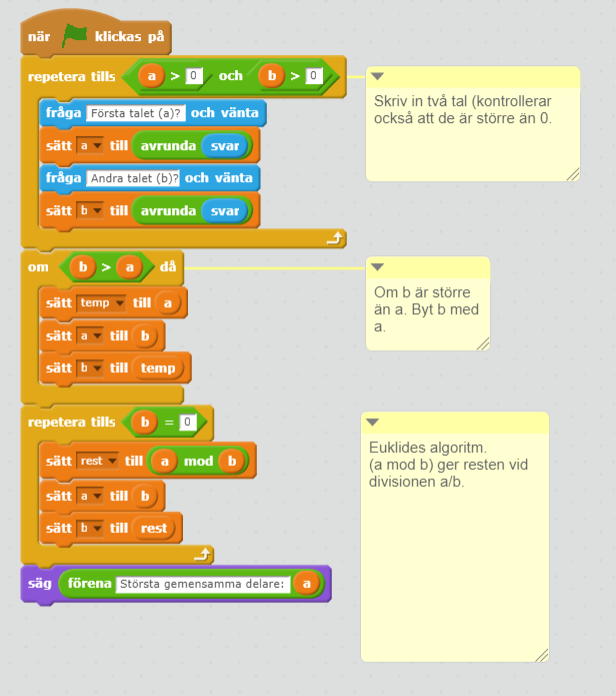
\includegraphics[scale=0.85]{euklidesimpl}

%\end{minipage}%
%\hfill%

Länk till projektet:  \\
 \url{https://scratch.mit.edu/projects/178445830/#editor }
\subsection{Uppgift 2: Binärsökning}
På denna uppgiften har vi en sorterad lista på 10 olika heltal.
Vi implementerade algoritmen rekursivt. Binärsökning använder en  \\
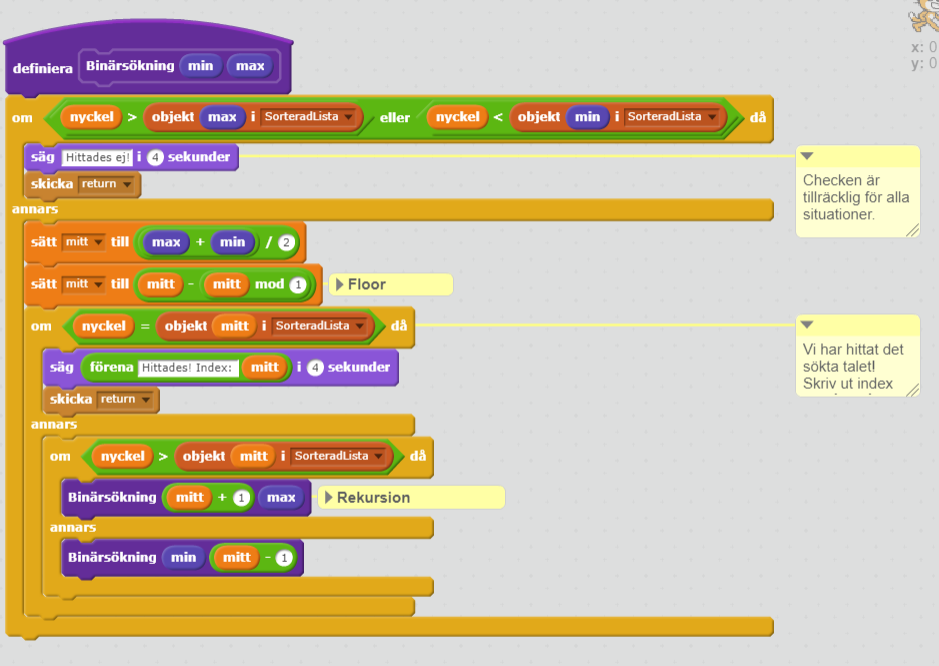
\includegraphics[scale=0.65]{binaryimpl}
\\ ``Definiera'' i Scratch liknar en metod i ett ``riktigt'' programmeringsspråk. Eftersom allt är globalt i Scratch fanns inget behov av att skicka med nyckeln eller array:n/listan.   \\
Länk till projektet: \\ \url{ https://scratch.mit.edu/projects/178458263/#editor }
\section{Tidrapport}
9/10 -2017 1h /person. 
10/10 - 2017 1h / person. 
\end{document}
